\section{Mateusz Mrowiec}
\label{sec:mmrowiec}

Zacznijmy od paru \underline{prostych} wzorów. Zaczynając od $e^{\pi i} = -1$ a następnie przechodząc do:
\[
\sum_{i=1}^\infty \frac{\frac{3}{4}\pi + i}{\sqrt{i^5+\frac{2}{7}i^3+1443-\sqrt[7]{16}}} = 0
\]

Tutaj chał bym dla odstresowania załączyć zdjęcie (Figure~\ref{fig:mysz}).

\begin{figure}[h]
\centering
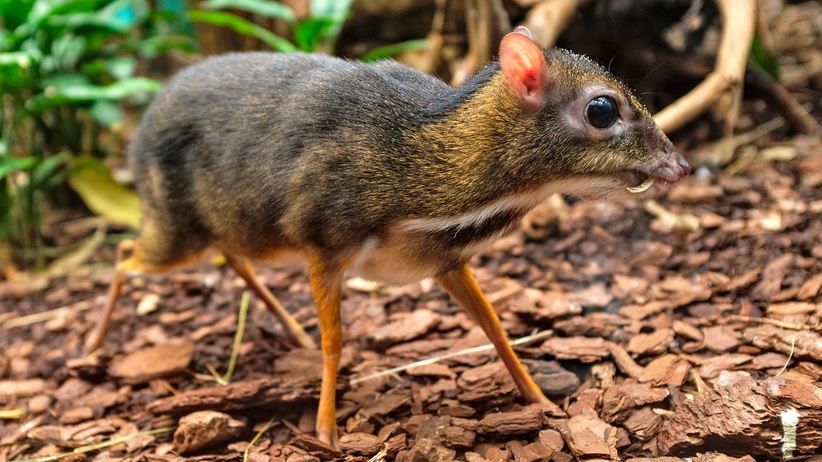
\includegraphics[width=0.5\textwidth]{pictures/Myszojelen.jpg}
\caption{Piękne zdjęcie słodkiego zwierzątka w lesie}
\label{fig:mysz}
\end{figure}

Pragnę również zacytować jeden z moich ulubionych tekstów.
\newline\newline
\textit{Lorem ipsum dolor sit amet, consectetur adipiscing elit. Morbi fringilla quis tortor ac efficitur. Curabitur mattis arcu ut elit malesuada sollicitudin. Fusce pharetra mattis commodo. Donec vulputate venenatis urna efficitur vestibulum. Mauris nec viverra augue, eu viverra turpis. Aenean vulputate tempus lobortis. Curabitur maximus turpis in leo pulvinar venenatis.}

\textit{Nullam vitae egestas velit, in ullamcorper velit. Praesent iaculis, justo vel tincidunt feugiat, mauris turpis ornare leo, non varius sem ipsum vehicula libero. Aenean a lectus id sapien tincidunt convallis consectetur sit amet dolor. Phasellus iaculis at lorem a ultricies. Curabitur ac odio eros. Aenean efficitur scelerisque quam. Ut feugiat massa ac ante lacinia, vel facilisis ligula tempor. In suscipit ac orci sed pretium. Praesent non purus at augue molestie vehicula. Suspendisse scelerisque libero et pellentesque accumsan. Donec venenatis volutpat commodo. Orci varius natoque penatibus et magnis dis parturient montes, nascetur ridiculus mus. Phasellus neque arcu, molestie fermentum nisl sed, varius rutrum erat. Vestibulum orci diam, cursus nec sollicitudin eu, sodales ut risus.}

\newpage

Chciał bym w tym miejscu wyciągnąć parę wniosków na podstawie zamieszczonej tabeli (Table~\ref{tab:and}). 
\begin{enumerate}
    \item Jeśli A jest prawdą i B jest prawdą to otrzymujemy \textbf{prawdę}.
    \item Jeśli A jest fałszem i B jest prawdą to otrzymujemy \textbf{fałsz}. 
    \item Jeśli A jest prawdą i B jest fałszem to otrzymujemy \textbf{fałsz}. 
    \item Na koniec jeśli A jest fałszem i B jest fałszem to oczywiście otrzymujemy \textbf{fałsz}. 
\end{enumerate}

\begin{table}[htbp]
\centering
\begin{tabular}{|c|c|c|}
\hline
A & B & $A\wedge B$ \\ \hline
1 & 1 & 1   \\ \hline
1 & 0 & 0   \\ \hline
0 & 1 & 0   \\ \hline
0 & 0 & 0   \\ \hline
\end{tabular}
\label{tab:and}
\caption{Tabla prawdy dla bramki AND.}
\end{table}

Zalety i wady bramki \emph{OR}\footnote{Wady i zalety są czysto subiektywnie i nie każdy będzie się z nimi zgadzał, warto aby każdy osobiście wyrobił sobie opinie na ten temat poprzez prace z bramkami.}:
\begin{itemize}
    \item[-] zwraca zero tylko w jednym przypadku
    \item[+] jest wstecznie kompatybilna z bramką \emph{AND} (też zwraca prawdę dla $A=1$ i $B=1$)
    \item[-] wejścia A i B mogą być zamienione miejscami i nie wpłynie to na działanie bramki
    \item[+] wejścia A i B mogą być zamienione miejscami jest to również zaleta
\end{itemize}




